\begin{figure*}[t]
  \centering
  \begin{subfigure}[t]{0.45\columnwidth}
    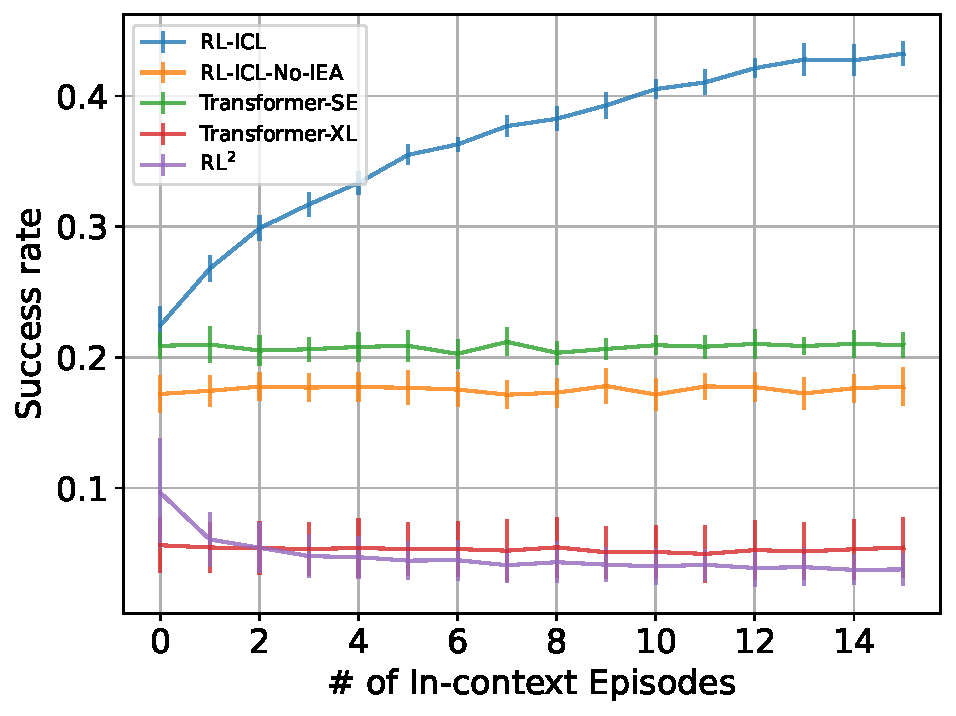
\includegraphics[width=\textwidth]{figures/results/icl_succ.pdf}
    \caption{Success Rate}
  \end{subfigure}
  \begin{subfigure}[t]{0.45\columnwidth}
    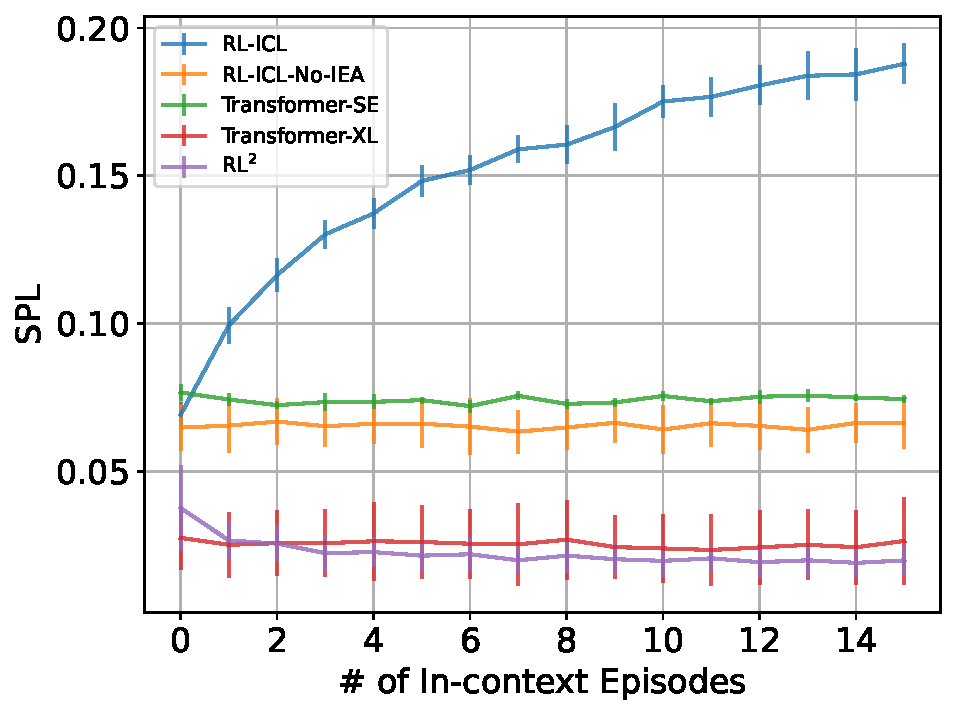
\includegraphics[width=\textwidth]{figures/results/icl_eff.pdf}
    \caption{Efficiency}
  \end{subfigure}
  \caption{
    Comparing the in-context learning capability of \method and baselines on \task. The number of episodes in the trial is displayed on the x-axis. The y-axis displays the success or efficiency at that episode count. Agents capable of in-context learning will increase in success and efficiency when encountering more episodes. Each method is run for 3 random seeds and evaluated on 10k distinct sequences. Error bars are standard deviations over trial outcomes between the 3 seeds.}
  \label{fig:icl-results}
\end{figure*}



\section{Experiments}
\label{sec:experiments} 

We first introduce the \Task (\task) task we use to study in-context learning for embodied navigation. Next, we analyze how \method enables in-context learning on this task and outperforms prior work and baselines. We then analyze ablations of \method and analyze its behaviors. We also show \method is capable of few-shot imitation learning. Finally, we show that \method outperforms the methods in \cite{lee2023supervisedpretraininglearnincontext} on the existing Darkroom and Miniworld tasks.

\subsection{\task: \Task}

To evaluate ICL capabilities for embodied agents, we introduce \task, an extension of the existing Object Navigation (\obnav) benchmark. \task assesses an agent's ability to find a sequence of objects in a house while operating from egocentric visual perception. For each object, the agent is randomly placed in a house and must locate and navigate to a specified object category. The agent used is a Fetch robot equipped with a $256 \times 256$ RGB head camera. Additionally, the agent possesses an odometry sensor to measure its relative displacement from the start of the episode. Navigation within the environment is executed through discrete actions: move forward 0.25 meters, turn left or right by 30 degrees, and tilt the camera up and down by 30 degrees. The agent also has a stop action, which ends the episode.

\task uses scenes from the Habitat Synthetic Scenes Dataset (HSSD)~\citep{khanna2023habitat} along with a subset of the YCB object dataset~\citep{calli2015ycb} containing 20 objects types. 
Note that \task requires navigating to \emph{small} objects unlike other \obnav variants that use large receptacles as goals \citep{habitat-challenge-2021}. This allows us to increase the dataset diversity by sampling objects randomly in the environment, unlike \obnav, where the receptacles are fixed parts of the scanned meshes. The random sampling also precludes the agent from using priors over object placements in scenes, forcing it to rely on the experience in its context.

\task defines a \emph{trial} as a sequence of episodes within a fixed home layout, where a home layout is defined by a combination of a floorplan, a furniture layout and set of object placements. A home layout contains on an average 22 objects where multiple object instances may be of the target category. Within an episode in the trial, a target object category is randomly selected and the agent is randomly placed in the house. The episode is successful if the agent calls the stop action within 2 meters of the object, with at least 10 pixels of the object in the current view. If the object is not found within $500$ steps the episode counts as a failure.

We evaluate the agents on unseen scenes from HSSD and report the success rate (SR) and Success-weighted by Path Length (SPL) metrics~\citep{anderson2018evaluation}. Specifically, we look at the SR and SPL of an agent as it accumulates more episodes in-context. Ideally, with more in-context episodes within a home layout, it should be more adept at finding objects and its SR and SPL should improve. See \Cref{sec:task-details} for further details on the \task.

\begin{figure*}[t]
  \centering
  \begin{subfigure}[t]{0.32\columnwidth}
    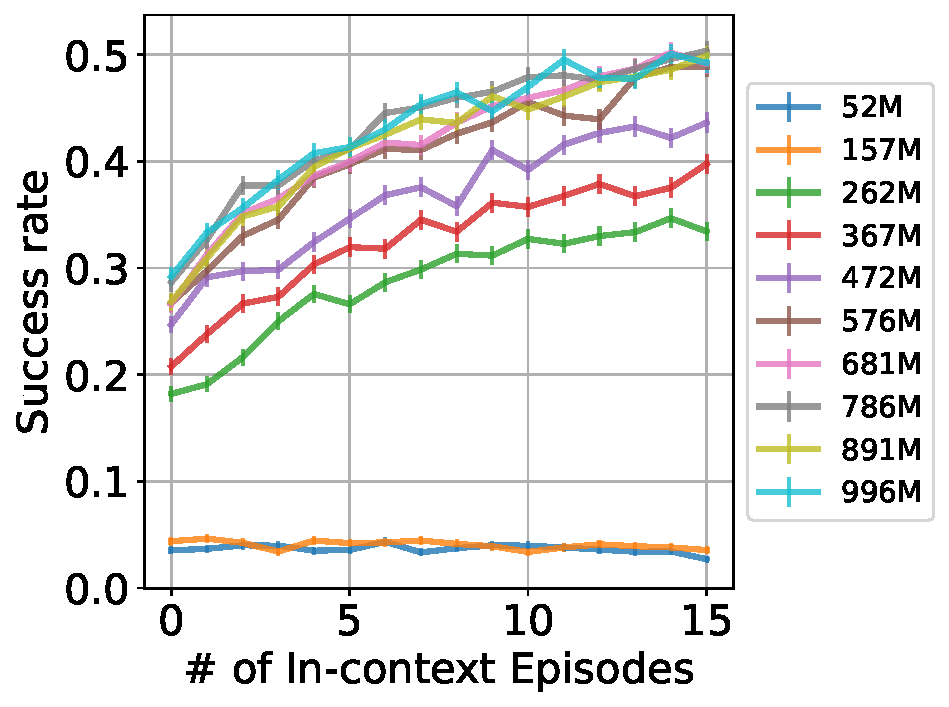
\includegraphics[width=\textwidth]{figures/results/train_icl_succ_15.pdf}
    \caption{Learning vs. ICL}
    \label{fig:icl-vs-updates} 
  \end{subfigure}
  \begin{subfigure}[t]{0.32\columnwidth}
    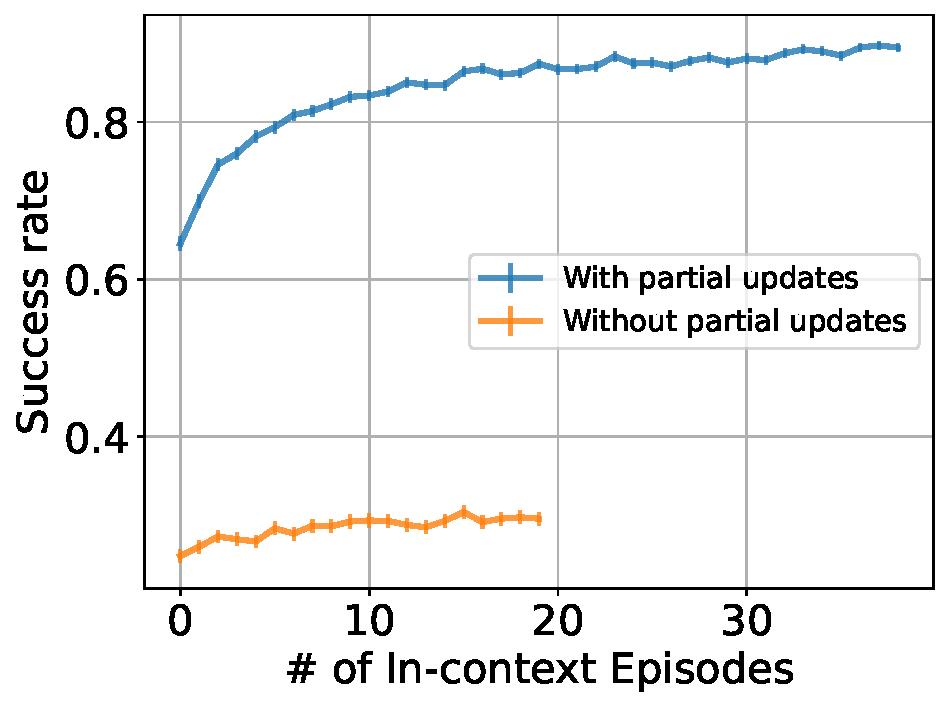
\includegraphics[width=\textwidth]{figures/results/partial_updates_custom_pddl_task_success.pdf}
    \caption{Update Scheme Ablation}
    \label{fig:updates} 
  \end{subfigure}
  \begin{subfigure}[t]{0.32\columnwidth}
    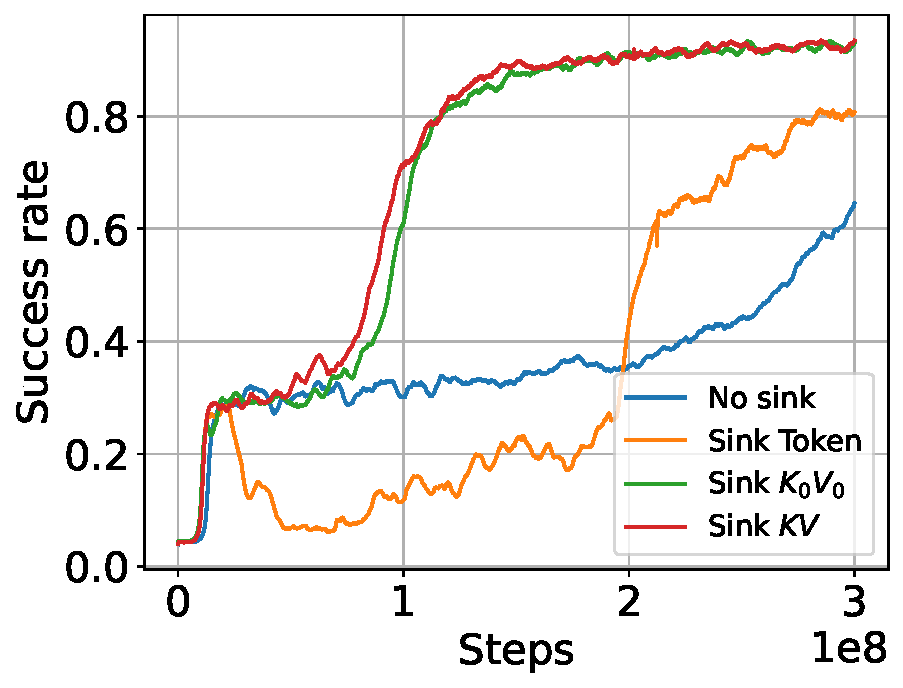
\includegraphics[width=\textwidth]{figures/results/sinktok_exps.pdf}
    \caption{Attention Sink Ablation}  
    \label{fig:sink-kv-learning-curve}
  \end{subfigure}
  \caption{
    Analyzing \method ICL capabilities.
    \cref{fig:icl-vs-updates} shows increased RL training results in agents that have a higher base success and stronger ICL capabilities with error bars giving standard error on the evaluation episodes.
    \cref{fig:updates} shows the partial updates are important in \method. 
    \cref{fig:sink-kv-learning-curve} shows \sinkv is important for learning speed and stability. 
    The results in Fig.\ref{fig:updates},\ref{fig:sink-kv-learning-curve} use the smaller ReplicaCAD scenes for easier analysis and thus have higher overall success rates. 
    These results performed on the easier ReplicaCAD scenes to save compute, so the numbers are higher overall.
  }
  \label{fig:analysis}
  \vspace*{-15pt}
\end{figure*}

\subsection{In-Context Learning on \task}
\label{sec:icl_on_task}

In this section, we compare the ability of \method and baselines to in-context learn in a new home layout. We compare \method to the following baselines:

\begin{itemize}[itemsep=2pt,topsep=0pt,parsep=0pt,partopsep=0pt,parsep=0pt,leftmargin=*]
  \item \textbf{\rls} \cite{duan2016rl}: Use an LSTM and keep the hidden state between trial episodes.
  \item \textbf{\trxl (TrXL)} \cite{dai2019transformerxl}: Use Transformer-XL and updates the constant-size memory recurrently. This is the model used in \cite{team2023human} trained in our setting. Following~\cite{team2023human} we use PreNorm \citep{gtrxl} and gating in the feedforward layers \citep{shazeer2020glu}. 
  \item \textbf{\ieafmethod}: \method without Inter-Episode Attention (IEA). Everything else, including the update scheme is the same as \method.
  \item \textbf{\semethod}: A transformer-based policy operating over only a single episode (SE) and without the update schemes from \method. 
\end{itemize}

All baselines are trained for 500M steps using a distributed version of PPO~\citep{wijmans2019dd}. Methods that utilize multi-episode context are trained with a context length of 4k, and use 8k context length during inference (unless mentioned otherwise, e.g. in our long-context experiments). The results in \Cref{fig:icl-results} demonstrate \method achieves better performance than baselines on 8k steps of ICL, achieving $ 43\%$ success rate v.s.  $ 22 \%$ success rate achieved by the closest performing baseline (\semethod).

Additionally, \method is able to effectively adapt to new home layouts throughout the course of the trial. In the first episode of the trial, transformer-based baseline methods attain a similar base performance of around $ 20 \%$ success rate. However, as more episodes arrive, the performance of \method increases. The recurrent models, Transformer-XL and \rls, have lower base performance at $10\%$ success rate and show no in-context learning. 
The performance of \rls degrades with more in-context episodes, which is aligned with the inability of the LSTM to model long sequences.


After 15 episodes of in-context experience, the success rate of \method increases from $ 23\%$ to $ 43\%$.  
The baselines do not possess this same ICL ability and maintain constant performance with subsequent in-context episodes.
\method also in-context learns to navigate faster to objects, as measured by the  gap in SPL.
As the trial progresses, the agent is able to more efficiently navigate to objects in the house with the SPL of \method increasing from $ 0.07$ to $ 0.188$. 
The baselines are unable to improve efficiency in-context and maintain a SPL of $ 0.025$ to $ 0.075$ throughout the entire trial.


\vspace{-5pt}
\subsection{\method Ablations and Analysis}
\label{sec:ablation}
\vspace{-5pt}



We demonstrate that the partial updates in \method and \sinkv are crucial to learning with RL over long context windows and acquiring ICL capabilities. We run these ablations in the smaller ReplicaCAD~\citep{szot2021habitat} scenes to make methods faster to train, but other details of the task remain the same.
We then show that ICL emerges later in the training and the context length in \method can be even further increased.

\textbf{No Partial Updates.} Firstly, we remove the partial updates in \method and find that it performs poorly (\Cref{fig:updates}), achieving $ 40 \%$ lesser SR at the first episode. This model also shows little ICL abilities with the SR only increasing $ 5 \% $ by the end of the trial versus a $ 25\%$ increase when using partial updates. 

\textbf{\sinkv.} Next, we demonstrate that using \sinkv is necessary for sample-efficient in-context RL learning. We trained the model on ReplicaCAD with and without attention sinks. The learning curves in \Cref{fig:sink-kv-learning-curve} shows that learning is more stable and faster with \sinkv which achieves 90\% success rate at 200M steps. It also shows that \sinkv performs similar to Softmax One \citep{off_by_one_softmax}, referred to as Sink $K_0V_0$. 
Without attention sink mechanisms, learning is slow and achieves less than 40\% success rate after 200M steps and reaching 64\% at 300M steps. Using sink token \citep{xiao2023efficient}, the training becomes unstable, achieving 40\% success rate at 200M steps training and reaching 80\% success rate at 300M steps. The details of the different sink attentions, their implementations and how the attention heads use the \sinkv can be found in \Cref{sec:app-sink-kv}.

\textbf{Training Steps v.s. ICL Abilities.} We find that \method only acquires ICL capabilities after sufficient RL training. As demonstrated in \Cref{fig:icl-vs-updates}, the agent is only capable of ICL after 157M steps of training. Models trained for 52M and 157M remain at constant success with more in-context experience. Further training does more than just increase the base agent performance in the first episode of the trial. 
From 262M steps to 367M steps, the agent base performance increases by $ 2\%$, yet the performance after 15 episodes of ICL performance increases $ 10 \%$.
This demonstrates that further training is not only improving the base capabilities of the agent to find objects, but also improving the agent's ability to utilize its context across long trials spanning many episodes.

\textbf{Context length generalization.} Next, we push the abilities of \method to in-context learn over contexts much larger than what is seen during training. In this experiment, we evaluate \method model, trained with 4k context length, on 32k steps of experience, which is enough to fit 80 episode trials in context. Assuming that the simulator is operating at 10Hz, this is almost 1 hour of agent experience within the context window. Note that for this experiment, we use our best checkpoint, which is trained for 1B steps. The results demonstrate that \method can generalize to contexts 8$\times$ larger at inference. \Cref{fig:ctx-gen} shows \method is able to further increase the success rate to over $ 55\% $ after 80 in context episodes and consistently maintains performance above $ 50 \% $ after 20 in-context episodes.

\textbf{64k steps trials.} Finally, we investigate scaling \textit{training} \method with 64k context length. We use the same hyperparameters as \cref{sec:icl_on_task}, but increase the number of partial updates per rollout such that the policy is updated every 256 steps, the same number of steps used in \method. \cref{fig:64k-train-succ} shows that the model can in-context learn over 175 episode and continue to improve success rate. More details are available at \Cref{sec:app-64k-train-eval}.

In \Cref{sec:per-obj} we analyze the performance of \method per object type. In \Cref{sec:app-what-agent-see} we qualitatively analyze what the agent attends to in successful and failure episodes. Finally, in \Cref{sec:shuffle-abl}, we show that not shuffling episodes in the context during training leads to worse performance.

\vspace{-5pt}
\subsection{Emergent Few-Shot Imitation Learning}
\vspace{-5pt}
\begin{figure*}[t]
  \centering
  \begin{subfigure}[t]{0.32\columnwidth}
    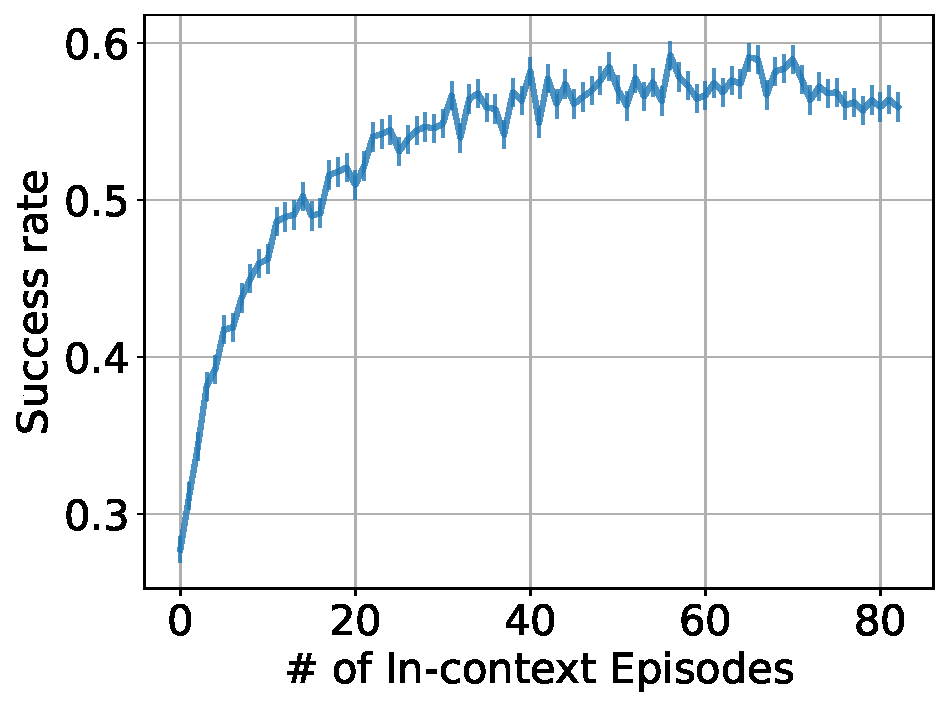
\includegraphics[width=\textwidth]{figures/results/ctx_gen_succ.pdf}
    \caption{Context Length Generalization}
    \label{fig:ctx-gen}
  \end{subfigure}
  \begin{subfigure}[t]{0.32\columnwidth}
    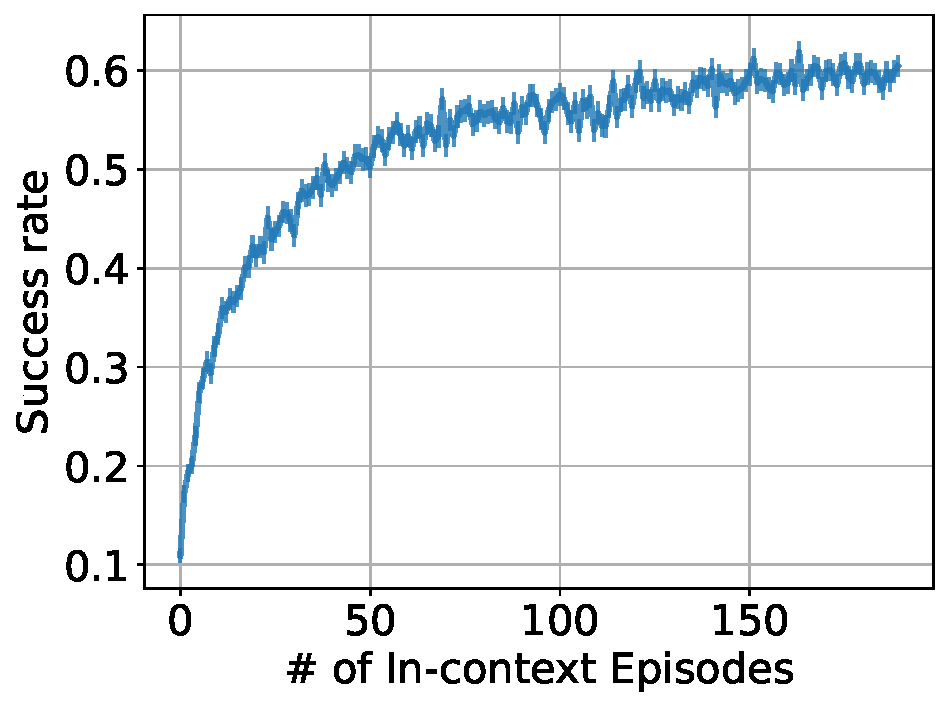
\includegraphics[width=\textwidth]{figures/results/64ksteps_training_inference_custom_pddl_task_success.pdf}
    \caption{64k Train Context Length}
    \label{fig:64k-train-succ}
  \end{subfigure}
  \begin{subfigure}[t]{0.32\columnwidth}
    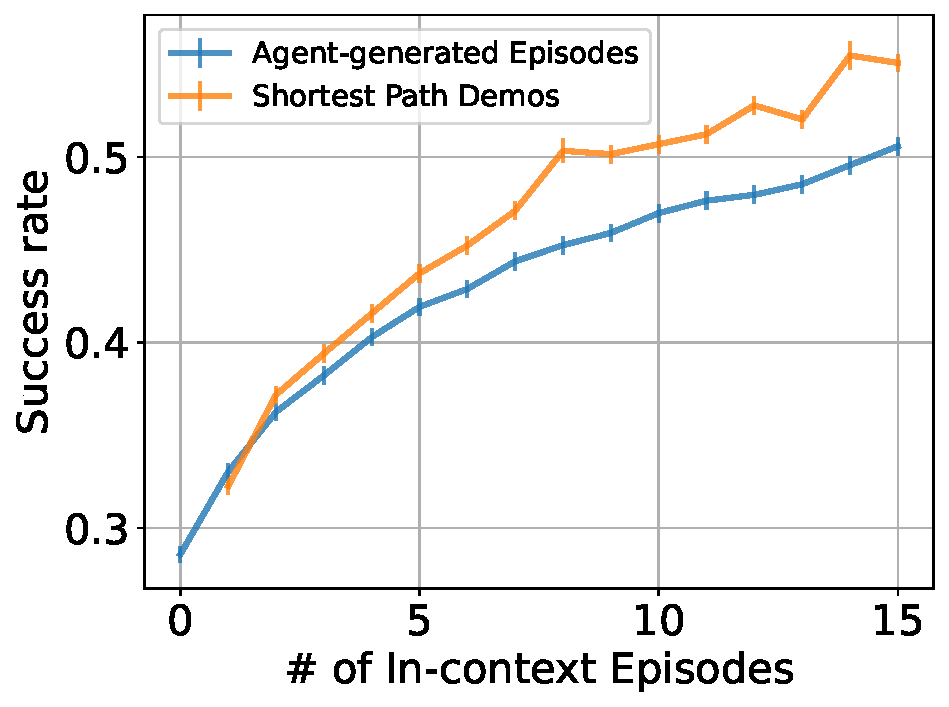
\includegraphics[width=\textwidth]{figures/results/fsil_succ.pdf}
    \caption{Few-Shot Imitation Learning}
    \label{fig:fsil}
  \end{subfigure}
  \vspace{-5pt}
  \caption{(a) \method trained with context length 4k generalizes to operating at 32k steps of in context experience in a new home layout. (b) \method trained at 64k context length shows ICL abilities over 175 episodes. (c) \method can do few-shot imitation learning despite not training for it. The error bars represent the standard error.}
  \vspace{-15pt}
\end{figure*}



In addition to learning in-context from self-generated experience in an environment, \method can also use its context to learn from demonstrations provided by an external agent or expert, despite never being trained on demonstrations and only learning from self-generated experience. 
We consider the setting of few-shot imitation learning \citep{duan2017one,wang2020generalizing} where an agent is given a set of trajectories $ \left\{ \tau_1, \dots,  \tau_N \right\} $ demonstrating behavior reaching desired goals $\left\{ g_1, \dots,  g_N \right\} $. The agent must then achieve a new $ g_{N+1}$ in new environment configurations using these demonstrations. 
\method is able to few-shot imitation learn by taking the expert demonstration as input via the context. Specifically, we generate $ N$ expert shortest path trajectories navigating to random objects from random start positions in an unseen home layout.
The success rate of these demos is around $ 80\%$ due to object occlusions hindering the shortest path agent from viewing the target object which is required for success.
These $ N$ trajectories are inserted into the context of \method and the agent is instructed to navigate to a new object in the environment. 

In \Cref{fig:fsil} we show that \method can utilize these expert demonstrations despite never seeing such shortest paths during training. \Cref{fig:fsil} shows the success rate of \method in a single episode after conditioning on some number of shortest path demonstrations. More demonstrations cover more of the house and the agent is able to improve navigation success.
We also compare to the success rate of an agent that has $ N$ episodes of experience in the house as opposed to $ N$ demonstrations. Using the demonstrations results in better performance with $ 5\%$ higher success rate for $ N=16$. 

\vspace{-5pt}
\subsection{Darkroom and Miniworld}
\label{sec:darkroom} 
\vspace{-5pt}

\begin{figure*}[t]
  \centering
  \begin{subfigure}[t]{0.32\columnwidth}
    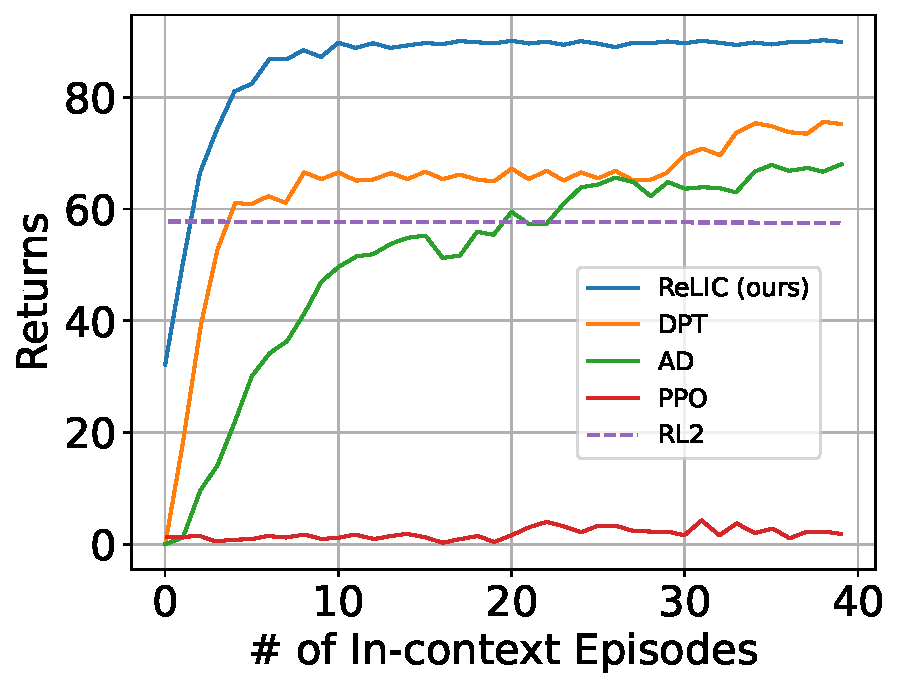
\includegraphics[width=\textwidth]{figures/results/darkroom_returns.pdf}
    \caption{Darkroom}
    \label{fig:dark_result}
  \end{subfigure}
  \begin{subfigure}[t]{0.32\columnwidth}
    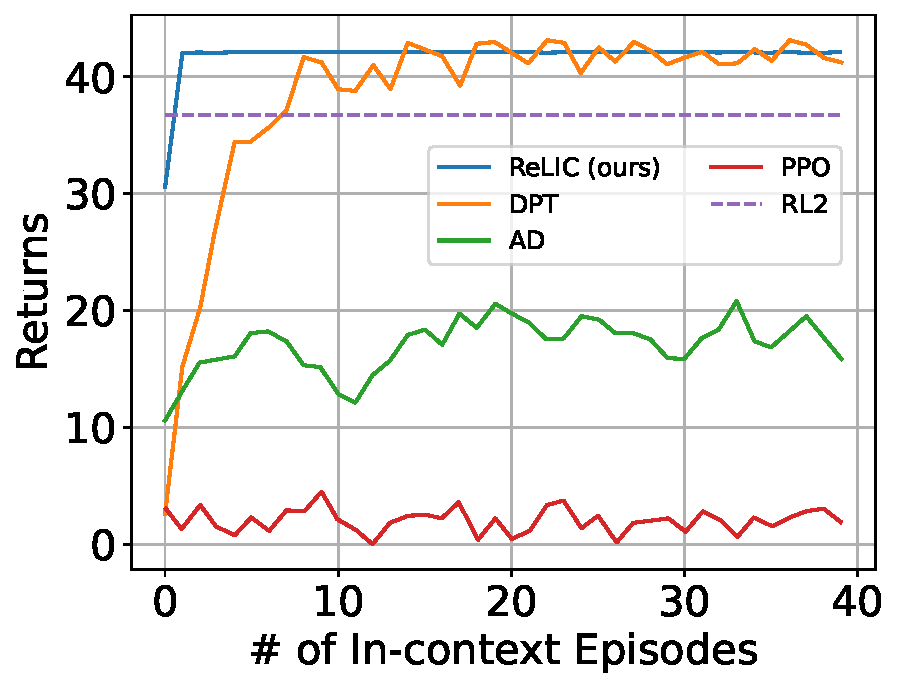
\includegraphics[width=\textwidth]{figures/results/miniworld_returns.pdf}
    \caption{Miniworld}
    \label{fig:mini_result}
  \end{subfigure}
  \vspace{-5pt}
  \caption{
    ICL comparison of \method and baselines in the Darkroom and Miniworld tasks. 
    \method has a higher base performance and adapts to new tasks with less experience. The baselines numbers are obtained from Figures 4b,d of \cite{lee2023supervisedpretraininglearnincontext}.
    } 
  \label{fig:dark_n_mini_result}
  \vspace{-10pt}
\end{figure*}

In this section, we evaluate \method on the Darkroom \citep{zintgraf2020varibadgoodmethodbayesadaptive} and Miniworld~\citep{gym_miniworld} environments and compare to the results from \cite{lee2023supervisedpretraininglearnincontext} to provide a comparison with existing baselines on these simpler benchmarks.
We directly take the numbers from \cite{lee2023supervisedpretraininglearnincontext} which include Decision-Pretrained Transformer (DPT), a supervised pretraining method for in-context meta-RL, Algorithm Distillation (AD) \citep{laskin2022context}, Proximal Policy Optimization (PPO) and \rls. 
\method is trained with context length 512, which fits 10 Miniworld and 5 Darkroom episodes. 
Policies are evaluated with 40 in-context episodes. 
Full details are in \Cref{sec:dark_n_min_hyperparams}.

\textbf{Darkroom.} \Cref{fig:dark_result} shows that \method outperforms all previous methods in the Darkroom task. Specifically, \method achieves base performance of 32 while the other methods have base performance lower than 2 returns. \method reaches 89 returns after 10 in-context episodes which is higher than 75 achieved by DPT after 39 in-context episodes.

\textbf{Miniworld.} \method has a higher base performance of 30 episode return compared to the best base performance of 10 as shown in \Cref{fig:mini_result}. It quickly reaches 42 returns after just 2 in-context episodes while DPT reaches the same result after 14 in-context episodes. \method also shows stable performance as the number of episodes increase compared to DPT which shows oscillation in the performance. 
In \Cref{sec:miniworld_abls}, we also show the importance of \sinkv and partial updates in both tasks.

